\documentclass[a4paper, 12pt, fleqn]{article}

\usepackage{amsmath}
\usepackage{amsthm}
\usepackage{amssymb}
\usepackage[margin=1in]{geometry}
\usepackage{xcolor}
\usepackage{float}
\usepackage{url}
\usepackage{array}
\usepackage{comment}
\usepackage[bookmarksnumbered=true,hypertexnames=false]{hyperref}
\usepackage{algorithm, algpseudocode}
\usepackage[capitalize,sort]{cleveref}

\hypersetup{
    colorlinks,
    linkcolor={red!50!black},
    citecolor={red!50!black},
    urlcolor={blue!50!black}
}

% THEOREMS

\newtheorem{theorem}{Theorem}
\newtheorem{definition}{Definition}
\newtheorem{example}{Example}
\newtheorem{corollary}{Corollary}[theorem]
\newtheorem{lemma}[theorem]{Lemma}

% SHORTHANDS

\newcommand*{\Th}{^{\textrm{th}}}
\newcommand*{\WLoG}{Without loss of generality}
\newcommand*{\wLoG}{without loss of generality}
\newcommand*{\wrt}{with respect to}

% SYMBOLS

\let\eps\epsilon
\newcommand*{\defeq}{:=}

% MATH

\newcommand*{\floor}[1]{\left\lfloor #1 \right\rfloor}
\newcommand*{\smallfloor}[1]{\lfloor #1 \rfloor}
\newcommand*{\ceil}[1]{\left\lceil #1 \right\rceil}
\newcommand*{\smallceil}[1]{\lceil #1 \rceil}
\newcommand*{\abs}[1]{\left\lvert #1 \right\rvert}
\newcommand*{\smallabs}[1]{\lvert #1 \rvert}
\newcommand*{\norm}[1]{\left\lVert #1 \right\rVert}
\newcommand*{\smallnorm}[1]{\lVert #1 \rVert}
\newcommand*{\Z}{\mathbb{Z}}
\DeclareMathOperator*{\E}{E}
\DeclareMathOperator*{\Var}{Var}
\DeclareMathOperator*{\argmin}{argmin}
\DeclareMathOperator*{\argmax}{argmax}
\DeclareMathOperator{\poly}{poly}
\DeclareMathOperator{\opt}{opt}
\newcommand*{\OPT}{\mathrm{OPT}}

% INITIALIZATIONS

\newcommand{\initMinimal}{
\setlength{\parindent}{0pt}
\setlength{\parskip}{0.5em}
}
\newcommand{\initFromContents}{
\tableofcontents
\newpage
\initMinimal{}
}
\newcommand{\initAfterBeginDocument}{
\maketitle
\initFromContents{}
}
\newcommand{\addMyBib}{
\bibliographystyle{plainurl}
\bibliography{bibdb}
}

\author{Eklavya Sharma}
\date{\empty}

\usepackage{diagbox}
\usepackage{tikz}
\usetikzlibrary{arrows.meta}

\title{Dominant Strategy Equilibria}

\begin{document}

\maketitle
\initMinimal{}

\begin{definition}
For a player $i$,
\begin{itemize}
\item action $a$ \emph{strongly dominates} action $b$ iff
\\ $u_i(a, s_{-i}) > u_i(b, s_{-i})$ for all $s_{-i} \in S_{-i}$.
\item action $a$ \emph{very weakly dominates} action $b$ iff
\\ $u_i(a, s_{-i}) \ge u_i(b, s_{-i})$ for all $s_{-i} \in S_{-i}$.
\item action $a$ \emph{weakly dominates} action $b$ iff
\\ $u_i(a, s_{-i}) \ge u_i(b, s_{-i})$ for all $s_{-i} \in S_{-i}$ and
\\ $u_i(a, s_{-i}) > u_i(b, s_{-i})$ for some $s_{-i} \in S_{-i}$.
\end{itemize}
\end{definition}

\begin{definition}
For a player $i$, action $a$ is a (strongly/weakly/very weakly) \textbf{dominant strategy} iff
$a$ (strongly/weakly/very weakly) dominates all others actions in $S_i$.
\end{definition}

\begin{definition}
A strategy profile $s^*$ is a (strongly/weakly/very weakly) \textbf{dominant strategy equilibrium}
(DSE) iff for each player $i \in N$, $s^*_i$ is a (strongly/weakly/very weakly) dominant strategy.
\end{definition}

\section{Examples}

\subsection{Prisoner's Dilemma}

Prisoner's Dilemma is a 2-player game where each player can either
cooperate ($C$) or betray ($B$). It has the following payoff matrix:

\begin{tabular}{|c|c|c|}
\hline
\diagbox{1}{2} & C & B
\\ \hline
C & $-2, -2$ & $-10, -1$
\\ \hline
B & $-1, -10$ & $-5, -5$
\\ \hline
\end{tabular}

\begin{theorem}
$(B, B)$ is a strongly dominant strategy equilibrium.
\end{theorem}
\begin{proof}
$u_1(C, C) = -2 < -1 = u_1(B, C)$ and
$u_1(C, B) = -10 < -5 = u_1(B, B)$.
Therefore, $B$ is a strongly dominant strategy for player 1.
By symmetry, $B$ is also a strongly dominant strategy for player 2.
Therefore, $(B, B)$ is a strong DSE.
\end{proof}

If we change the payoff matrix to the following,
$(B, B)$ will become a weak DSE:

\begin{tabular}{|c|c|c|}
\hline
\diagbox{1}{2} & C & B
\\ \hline
C & $-2, -2$ & $-10, -2$
\\ \hline
B & $-2, -10$ & $-5, -5$
\\ \hline
\end{tabular}

If we change the payoff matrix to the following,
all strategy profiles become very weak DSE, and no strategy profile is a weak DSE:

\begin{tabular}{|c|c|c|}
\hline
\diagbox{1}{2} & C & B
\\ \hline
C & $-2, -2$ & $-5, -2$
\\ \hline
B & $-2, -5$ & $-5, -5$
\\ \hline
\end{tabular}

\subsection{Braess Paradox}

Consider the following road network, where $n$ players wish to travel from $S$ to $T$,
and each player wants to minimize the time taken to travel from $S$ to $T$.

\begin{center}
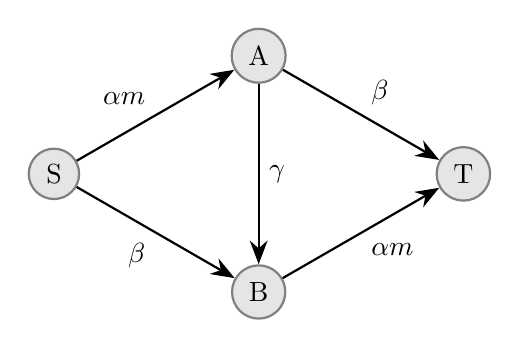
\begin{tikzpicture}[vertex/.style={circle,fill=black!10,draw=black!50,thick},
myedge/.style={-{Stealth[length=3mm]},thick},scale=1.0]
\node[vertex] (B) at (0, -1.5) {B};
\node[vertex] (A) at (0,  1.5) {A};
\node[vertex] (S) at (-2.6, 0) {S};
\node[vertex] (T) at ( 2.6, 0) {T};
\draw[myedge] (S) -- node[anchor=south east] {$\alpha m$} (A);
\draw[myedge] (A) -- node[anchor=south west] {$\beta$} (T);
\draw[myedge] (S) -- node[anchor=north east] {$\beta$} (B);
\draw[myedge] (B) -- node[anchor=north west] {$\alpha m$} (T);
\draw[myedge] (A) -- node[anchor=west] {$\gamma$} (B);
\end{tikzpicture}
\end{center}

The weight of an edge gives the time taken to traverse that edge.
Here $m$ is the number of vehicles using that road,
and $\alpha, \beta, \gamma$ are non-negative constants.
The utility of a player is the negative of the time taken to travel from $S$ to $T$.

Each player has the strategy set $\{A, B, AB\}$ (corresponding to the paths
$S \rightarrow A \rightarrow T$, $S \rightarrow B \rightarrow T$
and $S \rightarrow A \rightarrow B \rightarrow T$, respectively).
For a strategy profile $s$ and action $X$,
let $n_X(s)$ be the number of players who chose strategy $X$.
Note that $n_A(s) + n_B(s) + n_{AB}(s) = n$.
The utility function is given by
\[ u_i(s) = -\begin{cases}
\alpha(n_A(s) + n_{AB}(s)) + \beta & s_i = A
\\ \beta + \alpha(n_B(s) + n_{AB}(s)) & s_i = B
\\ \gamma + \alpha (n + n_{AB}(s)) & s_i = AB
\end{cases} \]

\begin{theorem}
\label{thm:braess-dse}
If $\gamma < \beta - \alpha n$, then $(AB)_{i \in N}$ is a
strongly dominant strategy equilibrium.
\end{theorem}
\begin{proof}
For any player, consider a strategy profile $s_{-i}$ for the other players. Then
\begin{align*}
& u_i(AB, s_{-i}) - u_i(A, s_{-i})
= (-u_i(A, s_{-i})) - (-u_i(AB, s_{-i}))
\\ &= (\alpha(n_A(s_{-i}) + 1 + n_{AB}(s_{-i})) + \beta)
    - (\gamma + \alpha(n + n_{AB}(s_{-1}) + 1))
\\ &= (\beta - \gamma) + \alpha(n_A(s_{-i}) - n)
\\ &\ge (\beta - \alpha n) - \gamma > 0
\end{align*}
\begin{align*}
& u_i(AB, s_{-i}) - u_i(B, s_{-i})
= (-u_i(B, s_{-i})) - (-u_i(AB, s_{-i}))
\\ &= (\beta + \alpha(n_B(s_{-i}) + 1 + n_{AB}(s_{-i})))
    - (\gamma + \alpha(n + n_{AB}(s_{-1}) + 1))
\\ &= (\beta - \gamma) + \alpha(n_B(s_{-i}) - n)
\\ &\ge (\beta - \alpha n) - \gamma > 0
\end{align*}
Therefore, for player $i$, action $AB$ is a strongly dominant strategy.
By symmetry, we get that $(AB)_{i \in N}$ is a strong DSE.
\end{proof}

Let $n = 1000$, $\alpha = 1/50$, $\beta = 25$ and $\gamma = 0$.
By \cref{thm:braess-dse}, $(AB)_{i \in N}$ is a strong DSE.
Then for each player, the utility of the DSE is $-(\gamma + 2\alpha n) = -40$.
Let $s^*$ be the strategy profile where half the players play $A$ and the others play $B$.
Then for each player $i$, $u_i(s^*) = -(\beta + \alpha n/2) = -35$.
Therefore, the utility of $s^*$ is higher than that of the strong DSE.

\subsection{Second-price Auction}

Consider a second-price auction with $n$ players.
Let $v_i$ and $b_i$ be the valuation and bid, respectively, of player $i$.

Let $y_i(b)$ be 1 iff player $i$ wins for the bid profile $b$ and 0 otherwise.
Let $t(b)$ be the second-highest bid in $b$ (if there are multiple highest bids,
they are also second-highest bids).
Then $u_i(b) = y_i(b)(v_i - t(b))$.

\begin{lemma}
For every player $i$, $b_i = v_i$ is a weakly dominant strategy.
\end{lemma}
\begin{proof}
Consider any $b_i \neq v_i$.
We will first show that $v_i$ very weakly dominates $b_i$.
Let $b_{-i}$ be any bid profile of the other players.

For any $x \in \mathbb{R}$, we get
\[ y_i(x, b_{-i}) = 1 \implies x \ge \max(b_{-i}) = t(x, b_{-i}) \]
\[ y_i(x, b_{-i}) = 0 \implies x \le \max(b_{-i}) \]
\textbf{Case 1a}: $y_i(v_i, b_{-i}) = 1$ and $y_i(b_i, b_{-i}) = 1$.
\[ \implies t(v_i, b_{-i}) = \max(b_{-i})
\quad\textrm{and}\quad t(b_i, b_{-i}) = \max(b_{-i}) \]
\[ \implies u_i(v_i, b_{-i}) = v_i - t(v_i, b_{-i}) = v_i - \max(b_{-i})
    = v_i - t(b_i, b_{-i}) = u_i(b_i, b_{-i}) \]
\textbf{Case 1b}: $y_i(v_i, b_{-i}) = 1$ and $y_i(b_i, b_{-i}) = 0$.
\[ \implies v_i \ge t(v_i, b_{-i}) = \max(b_{-i}) \]
\[ \implies u_i(v_i, b_{-i}) = v_i - t(v_i, b_{-i}) \ge 0 = u_i(b_i, b_{-i}) \]
\textbf{Case 2a}: $y_i(v_i, b_{-i}) = 0$ and $y_i(b_i, b_{-i}) = 1$.
\[ \implies v_i \le \max(b_{-i}) = t(b_i, b_{-i}) \le b_i \]
\[ \implies u_i(v_i, b_{-i}) = 0 \ge v_i - t(b_i, b_{-i}) = u_i(b_i, b_{-i}) \]
\textbf{Case 2b}: $y_i(v_i, b_{-i}) = 0$ and $y_i(b_i, b_{-i}) = 0$.\\
Then $u_i(v_i, b_{-i}) = 0 = u_i(b_i, b_{-i})$.

Since $u_i(v_i, b_{-i}) \ge u_i(b_i, b_{-i})$ for all $b_{-i}$,
$v_i$ very weakly dominates $b_i$.

We will now show that $v_i$ weakly dominates $b_i$.
Consider the profile $b_{-i}$ where all players other than $i$ bid $(v_i + b_i) / 2$.

\textbf{Case 1}: $b_i > v_i$.\\
Then player $i$ wins with bid $b_i$ and loses with bid $v_i$,
so $u_i(v_i, b_{-i}) = 0$ and
\[ u_i(b_i, b_{-i}) = v_i - \frac{v_i + b_i}{2} = \frac{v_i - b_i}{2} < 0. \]
Therefore, $u_i(v_i, b_{-i}) > u_i(b_i, b_{-i})$.

\textbf{Case 2}: $v_i > b_i$.\\
Then player $i$ wins with bid $v_i$ and loses with bid $b_i$,
so $u_i(b_i, b_{-i}) = 0$ and
\[ u_i(v_i, b_{-i}) = v_i - \frac{v_i + b_i}{2} = \frac{v_i - b_i}{2} > 0. \]
Therefore, $u_i(v_i, b_{-i}) > u_i(b_i, b_{-i})$.
\end{proof}

\begin{corollary}
For second-price auctions, the bid profile $(v_1, v_2, \ldots, v_n)$ is a weak DSE.
\end{corollary}

\section{Properties of DSE}

\begin{lemma}
\label{thm:no-weak-dom-strategy}
For any player, there cannot be two distinct weakly dominant strategies.
\end{lemma}
\begin{proof}
Assume player $i$ has two distinct weakly dominant strategies $a$ and $b$.
Since $a$ weakly dominates $b$, $\exists s_{-i} \in S_{-i}$ such that
$u_i(a, s_{-i}) > u_i(b, s_{-i})$.
Since $b$ weakly dominates $a$, $u_i(b, s_{-i}) \ge u_i(a, s_{-i})$.
This is a contradiction, so for any player,
there cannot be two distinct weakly dominant strategies.
\end{proof}

\begin{theorem}
There is at most one weak DSE for a strategic form game.
\end{theorem}
\begin{proof}
Assume there are two distinct weak DSEs $s$ and $t$ for a strategic form game.
Since $s \neq t$, there is a player $i$ such that $s_i \neq t_i$.
Since $s$ and $t$ are weak DSEs, $s_i$ and $t_i$ are weakly dominant strategies for player $i$.
But this contradicts \cref{thm:no-weak-dom-strategy}.
\end{proof}

%\addMyBib{}

\end{document}
